\section{Kombinatorik}
\label{sec:kombinatorik}
\subsection{Vier Elementare Abzählprobleme}
\label{sec:vier-elementare-abzahlp}
Bei allen vier folgenden Abzählproblemen geht es um eine Auswahl von $k$ Elementen aus einer Gesamtheit von
$n$ Objekten. Man teilt die Probleme nach zwei Kriterien ein:
\begin{itemize}
    \item Spielt in der Auswahl die Reihenfolge der Elemente eine Rolle?
    \item Sind Wiederholungen der Elemente erlaubt?
\end{itemize}
Eine Auswahl von $k$ Objekten aus $n$ Objekten bei der die Reihenfolge eine Rolle spielt, 
heisst \textbf{Variation} von $k$ Objekten aus $n$. 
Eine Auswahl von $k$ Objekten aus $n$ Objekten bei der die Reihenfolge keine Rolle spielt, 
nennt man \textbf{Kombination} von $k$ Objekten aus $n$ Objekten.
\begin{itemize}
    \item Variationszahl ohne Wiederholung: $\frac{n!}{(n-k)!}$
    \item Variationszahl mit Wiederholung: $n^k$
    \item Kombinationszahl ohne Wiederholung: $\binom{n}{k} = \frac{n!}{k!(n-k)!}$
    \item Kombinationszahl mit Wiederholung: $\binom{n+k-1}{k} = \frac{(n+k-1)!}{k!(n-1)!}$
\end{itemize}
\subsection{Binomialkoeffizient}
\label{sec:binomialkoeffizient}
Die \textbf{Fakultät} $n!$ ist für eine natürliche Zahl $n$ rekursiv definiert. Für den Startwert $0$ als $0!=1$ 
und für jeden Nachfolger $n\ geq 1$ definiert man $n! = n \cdot (n-1)!$ \\
Der Binomialkoeffizient $\binom{n}{k}$ ist für natürliche Zahlen $0 \leq k \leq n$ definiert als
\begin{equation*}
    \binom{n}{k} = \frac{n!}{k! \cdot (n-k)!}
\end{equation*}
Allgemein gilt die folgende Konstruktionsformel der Binomialkoeffizienten:
\begin{equation*}
    \binom{n+1}{k+1} = \binom{n}{k} + \binom{n}{k+1}
\end{equation*}
\subsubsection{Pascal'sches Dreieck}
\begin{center}
    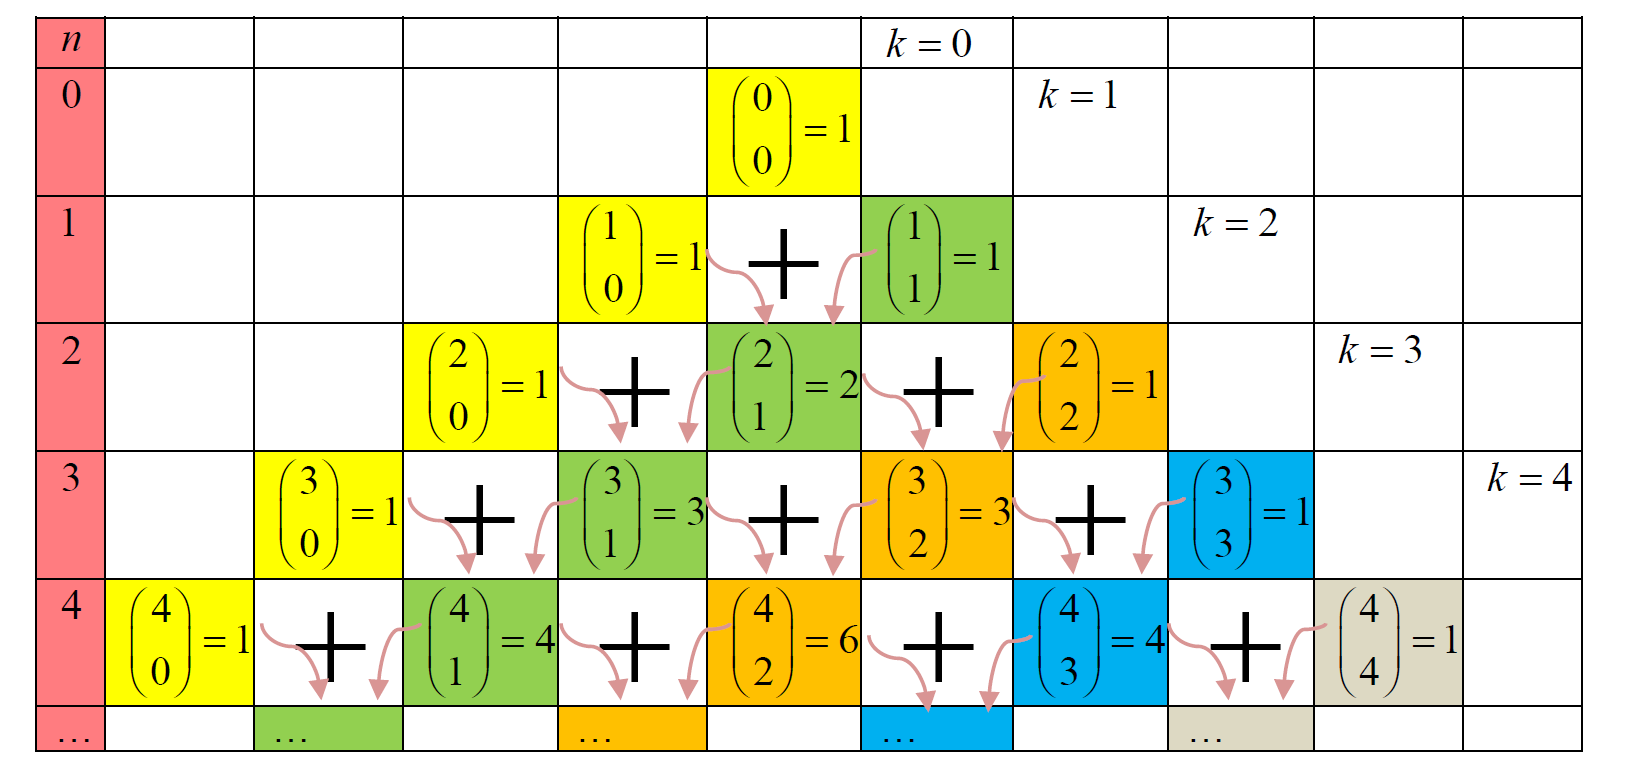
\includegraphics[width=1\textwidth]{images/pascal.png}
\end{center}
Die absteigenden Diagonalen von rechts nach links gehören jeweils zum gleichen $k$ Wert. 
Sie sind in der gleichen Farbe gehalten. Die Zeilen gehören jeweils zu einem bestimmten $n$ Wert. 
Man beachte, wie die Einträge jeder Zeile aus den Werten der jeweils vorhergehenden Zeile nach obiger Formel berechnet werden.
\subsubsection{Wichtige Eigenschaften der Binomialkoeffizienten}
\label{sec:wichtige-eigenschaften-der-binomialkoeffizienten}
\begin{itemize}
    \item Leere Menge: $\binom{n}{0} = 1$
    \item Symmetrie: $\binom{n}{k} = \binom{n}{n-k}$
    \item Rekursion: $\binom{n+1}{k+1} = \binom{n}{k} + \binom{n}{k+1}$
    \item Binomischer Lehrsatz: $(a+b)^n = \binom{n}{0}a^0b^n + \binom{n}{1}ab^{n-1} + \binom{n}{2}a^2b^{n-2} + \cdots + \binom{n}{n-1}a^{n-1}b + \binom{n}{n}a^nb^0 = 
        \sum_{k=0}^n \binom{n}{k}a^kb^{n-k}$ Für komplexe Zahlen $a$, $b$ $\in \mathbb{C}$
    \item Summe: $\sum^n_{k=0} \binom{n}{k} = \binom{n}{0} + \binom{n}{1} + \binom{n}{2} + \cdots + \binom{n}{n} = 2^n$
\end{itemize}